%!TEX TS-program = xelatex

% -- Document Class -----------------------------------------------------------

\documentclass[a4paper, 12pt]{article}

% -- Packages -----------------------------------------------------------------

% Language
\usepackage{polyglossia}
    \setmainlanguage{english}
    \setotherlanguage{german}
% Context sensitive quotation
\usepackage{csquotes}
% Citations
\usepackage[style=alphabetic, backend=biber]{biblatex}
    \addbibresource{References.bib}
% Customize enumerations
\usepackage{enumitem}
% Extend options for positioning floats
\usepackage{float}
% Support highlighting of certain parts of the text
\usepackage{framed}
% Support spaces in filenames
\usepackage{grffile}
% Tools for mathematical typesetting
\usepackage{mathtools}
% Headers & Footers
\usepackage[automark, nouppercase]{scrpage2}
% Emphasize text
\usepackage{soul}
% To change the format of titles
\usepackage{titlesec}
% Support for unicode math fonts
\usepackage{unicode-math}
% Extended color support
\usepackage[x11names]{xcolor}
% Extras for XƎTEX
\usepackage{xltxtra}
% Hyperlinks and pdf properties
\usepackage{hyperref}

% -- Color Definitions --------------------------------------------------------

% Background color for syntax highlighting
\definecolor{bgcolor}{rgb}      {1,     1,      1}

% Custom color definitions
\definecolor{aqua}{rgb}         {0,     0.56,   1}
\definecolor{bluegray}{rgb}     {0.22,  0.46,   0.84}
\definecolor{grape}{rgb}        {0.56,  0,      1}
\definecolor{lightgray}{rgb}	{0.94,	0.94,	0.94}
\definecolor{orchid}{rgb}       {0.41,  0.13,   0.55}
\definecolor{orange}{rgb}       {1,     0.54,   0}
\definecolor{silver}{rgb}       {0.57,  0.57,   0.57}
\definecolor{turquoise}{rgb}    {0,     0.86,   0.84}

% -- Macros -------------------------------------------------------------------

\newcommand{\Title}{Exercises}
\newcommand{\TitleDescription}{Computer Aided Verification}
\newcommand{\Version}{1}
\newcommand{\Subject}
    {Solutions for the exercises of the course Computer Aided Verification}
\newcommand{\KeyWords}{BDD, Kripke structure}
\newcommand{\LeftFooter}{\Title~—~\TitleDescription}

\newcommand{\AuthorOne}{René Schwaiger}
\newcommand{\MailOne}{\href{mailto:sanssecours@f-m.fm}{sanssecours@f-m.fm}}

% Syntax highlighting definitions
% Text
\newcommand{\hlstd}[1]{\textcolor{black}{#1}}
% Numbers
\newcommand{\hlnum}[1]{\textcolor{DarkOrchid4}{#1}}
\newcommand{\hlesc}[1]{\textcolor[rgb]{1,0,1}{#1}}
% Strings
\newcommand{\hlstr}[1]{\textcolor{SeaGreen3}{#1}}
\newcommand{\hlpps}[1]{\textcolor[rgb]{0.51,0.51,0}{#1}}
% Comments
\newcommand{\hlslc}[1]{\textcolor{aqua}{#1}}
\newcommand{\hlcom}[1]{\textcolor{aqua}{#1}}
\newcommand{\hlppc}[1]{\textcolor[rgb]{0,0.51,0}{#1}}
\newcommand{\hlopt}[1]{\textcolor[rgb]{0,0,0}{#1}}
\newcommand{\hllin}[1]{\textcolor[rgb]{0.33,0.33,0.33}{#1}}
% Keywords
\newcommand{\hlkwa}[1]{\textcolor{DodgerBlue3}{#1}}
\newcommand{\hlkwb}[1]{\textcolor[rgb]{0,0.34,0.68}{#1}}
\newcommand{\hlkwc}[1]{\textcolor{DarkOrchid4}{#1}}
% Functions
\newcommand{\hlkwd}[1]{\textcolor{orange}{#1}}

\newcommand{\codeinput}[1]
{
    \begin{leftbar}
        {\fontsize{9pt}{11pt}\input{Code/#1}}
    \end{leftbar}
}

\newcommand{\code}[1]
{
    \hl{\texttt{#1}}
}

% -- Document Properties ------------------------------------------------------

% Background color for highlighted text
\sethlcolor{lightgray}

% No indentation after paragraphs
\setlength\parindent{0cm}

% Hyperref properties
\hypersetup
{
    pdftitle    = {\Title},
    pdfsubject  = {\Subject},
    pdfauthor   = {\AuthorOne},
    pdfkeywords = {\KeyWords},
    colorlinks  = true,
    linkcolor   = black,
    anchorcolor = black,
    citecolor   = silver,
    urlcolor    = orange
}

% -- Fonts --------------------------------------------------------------------

% Use same size for numbers and other text
\defaultfontfeatures{Numbers=Lining}

% Set fonts for document
\setmainfont[Mapping=tex-text]{Avenir Next}
\setsansfont[Mapping=tex-text]{Ubuntu}
\setmonofont[Scale=MatchLowercase]{Menlo}
\setmathfont{Asana-Math.otf}
\setmathfont[range=\mathtt, Scale=MatchLowercase]{Menlo}

% Define font styles
\newfontfamily\Zapfino{Zapfino}

% -- Header And Footers -------------------------------------------------------

% Use normal font instead of italic font for head
\renewcommand{\headfont}{\normalfont}

% Set headers and footers
\ihead{\headmark}
\ohead{}
\ifoot{\LeftFooter}
\ofoot{\thepage}

% Set height of head
\setlength{\headheight}{1.8\baselineskip}

% Set thickness of separation line in header, footer
\setheadsepline{0.5pt}
\setfootsepline{0.5pt}

% -- Titlepage ----------------------------------------------------------------

\pagestyle{empty}
\begin{document}

\begin{titlepage}
    \begin{center}
        % Title and title-description
        {\Huge\Zapfino\Title}
        \vskip 0.5cm
        {\color{aqua}\hrule}
        \vskip 0.5cm
        {\Large\textit\TitleDescription}
        \vskip 14cm
    \end{center}

    % Date and version number
    \begin{leftbar}
        \begin{tabular}{ll}
            \textbf{Author}  & \AuthorOne\\
            \textbf{Mail}    & \MailOne\\
            \textbf{Version} & \Version\\
            \textbf{Date}    & \today
        \end{tabular}
    \end{leftbar}

\end{titlepage}


% -- Table of Contents --------------------------------------------------------

% Set section format for table of contents
\titleformat{\section}{\sffamily\bfseries}{}{0pt}{}[{\color{aqua}\hrule}]

% Set separation of dots between name of section and page number to such a high
% value that there will be no points in the table of contents
\makeatletter \renewcommand{\@dotsep}{10000} \makeatother
% Use blank header and footer
\pagestyle{empty}
% Start on new page
\newpage
% The table of contents starts at the second page
\setcounter{page}{2}
% Set table of contents
\tableofcontents

% -- Section & Paragraph Style ------------------------------------------------

% Set format for section
\titleformat{\section}
    {\large\sffamily\bfseries}  % Large, bold, sans serif font for section
    {}                          % No format applied to whole title
    {0pt}                       % No separation between label and title
    {\thesection~·~}            % Start with section number
    [{\color{aqua}\hrule}]      % Underline with blue ruler

% Set format for other sections and paragraphs
% Color = orchid, Font = bold, sans serif
\titleformat*{\subsection}{\color{orchid}\sffamily\bfseries}
\titleformat*{\subsubsection}{\color{orchid}\sffamily\bfseries}
\titleformat*{\paragraph}{\color{orchid}\sffamily\bfseries}
\titleformat*{\subparagraph}{\color{orchid}\sffamily\bfseries}

% -- Page Style ---------------------------------------------------------------

% Start with text on a new page
\newpage
% Display headers and footers
\pagestyle{scrheadings}

% -- Text ---------------------------------------------------------------------

\section{Binary Decision Diagrams}

\subsection{Exercise 1}

Give a linear time algorithm for BDD isomorphism as defined on page 9.

\subsubsection{Solution}

\codeinput{bdd}

\newpage
\subsection{Exercise 2}

Describe a size-efficient BDD for the relation “a ≥ b” for n-bit integer
numbers.

\subsubsection{Solution}

We already know that related variables should be close together in the
ordering. Therefore we place the bits of the same significance after each
other starting from the most significant bit of $a$. This leaves us with the
ROBDD shown in Figure~\ref{figure:OBDD_Comparison}.

\begin{figure}[htbp]
    \centering
        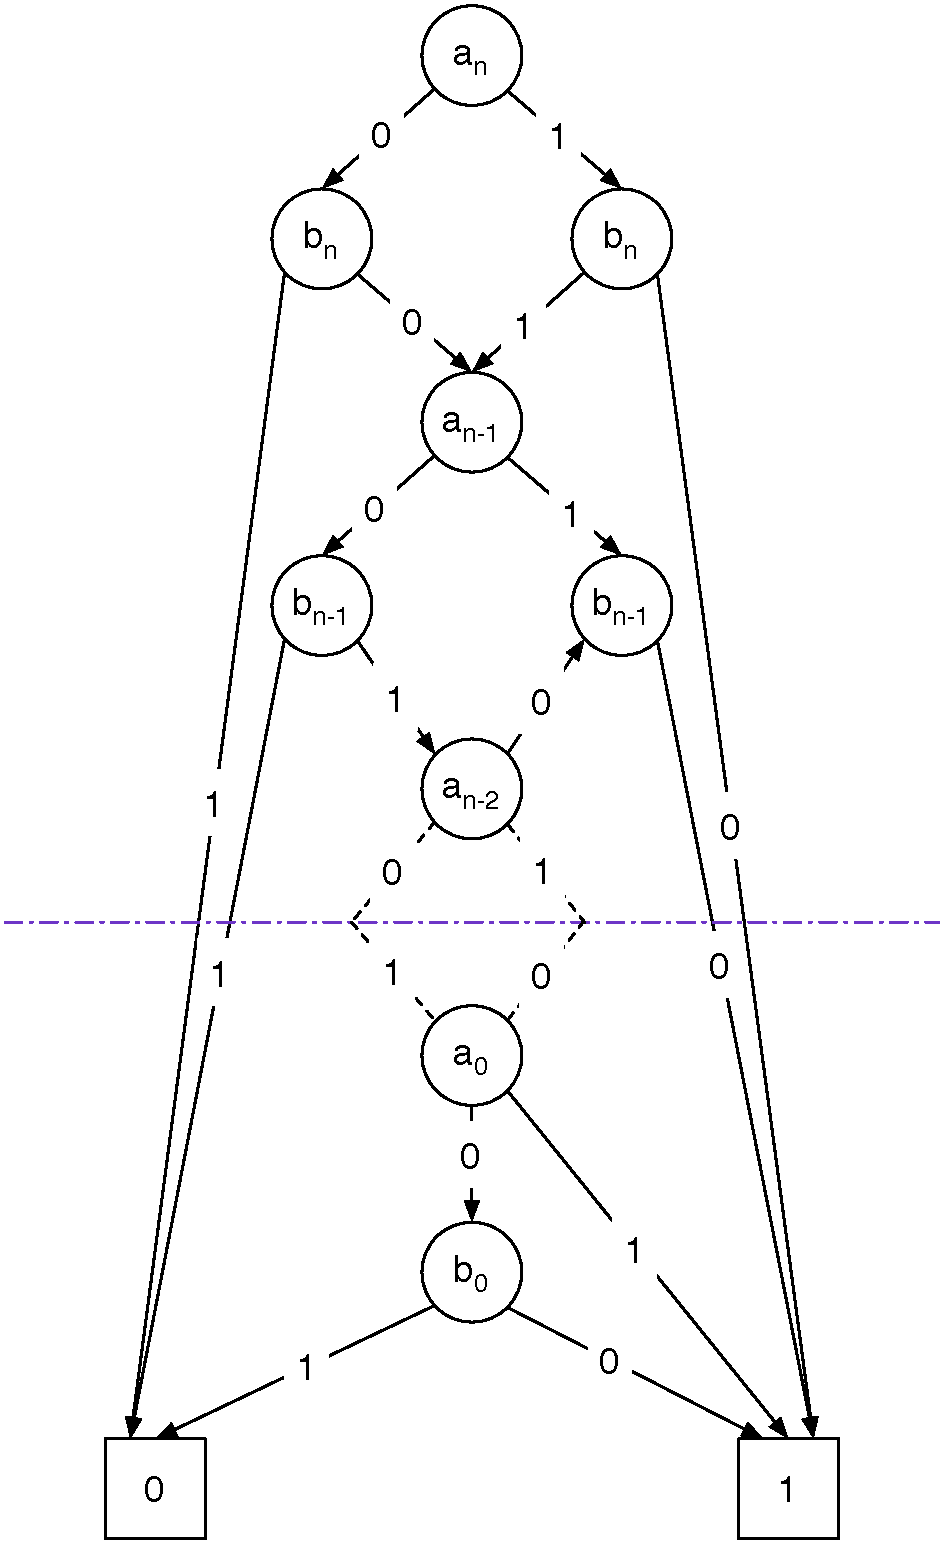
\includegraphics[width=.62\textwidth]{Figures/OBDD Comparison.pdf}
    \caption{OBDD for the relation “a ≥ b”}
    \label{figure:OBDD_Comparison}
\end{figure}

\subsection{Exercise 3}

Describe an algorithm which transforms a BDD into an equivalent boolean
formula.

\subsubsection{Solution}

The following code shows an algorithm which creates a boolean formula in
disjunctive normal form. The basic idea behind the code is to create a
conjunction of every variable visited on a path to a terminal node with value
“1”. We create the whole DNF-formula by joining the formulas for these paths
by disjunction.

\codeinput{bdd_to_formula}

\section{Temporal Logic}

\subsection{Exercise 4}

Prove the equivalence for $\mathbf{A}(f \mathbf{U} g)$ on page 16.

\subsubsection{Solution}

We need to prove that $\mathbf{A}(f \mathbf{U} g)$ is equivalent to $¬E(¬g
\mathbf{U} ¬f ∧ ¬g) ∧ ¬\mathbf{EG} ¬g$. We use the following equivalences:

\begin{enumerate}[label=(\arabic*)]
    \item $\mathbf{A} f ⇔ ¬\mathbf{E}¬f$
    \item $¬(f \mathbf{U} g) ⇔ (\mathbf{G}¬g ∨ ¬g \mathbf{U} ¬f ∧ ¬g)$
    The formula above is true since for $f$ until $g$ to not hold:
        \begin{enumerate}

            \item $g$ has to not hold at all (there exists no $k$ such that
            $π^k⊧g$) or

            \item $f$ might hold at first, while $g$ does not hold, but $g$
            does not hold after that ($¬g \mathbf{U} ¬f ∧ ¬g$).

        \end{enumerate}

    \item $\mathbf{E}(f ∨ g) ⇔ \mathbf{E}f ∨ \mathbf{E}g$
    \item $¬ (f ∨ g) ⇔ ¬f ∧ ¬g$
\end{enumerate}

to deduct the following proof:
\begin{align*}
    \mathbf{A}\left(f \mathbf{U} g\right)
    & \stackrel{(1)}{⇔} ¬\mathbf{E} ¬\left(f\mathbf{U} g\right)\\
    & \stackrel{(2)}{⇔} ¬\mathbf{E} \left(\left(\mathbf{G}¬g\right) ∨
      \left(¬g\mathbf{U} ¬f ∧ ¬g\right)\right)\\
    & \stackrel{(3)}{⇔} ¬\left(\mathbf{EG}¬g ∨
      \mathbf{E}\left(¬g\mathbf{U} ¬f ∧ ¬g\right)\right)\\
    & \stackrel{(4)}{⇔} ¬\mathbf{EG}¬g ∧ ¬\mathbf{E}\left(¬g\mathbf{U} ¬f ∧
      ¬g\right)\\
\end{align*}

\subsection{Exercise 5}

Show the following lemma: Let $M$ and $N$ be two Kripke structures such that
the transition relation of $M$ is a superset of the transition relation of
$N$. If an LTL property $f$ holds on $M$, then $f$ also holds on $N$.

\subsubsection{Solution}

Let us assume that a certain LTL formula $\mathbf{A}f$ holds on $M$. Since the
transition relation of $M$ is a superset of the transition relations of $N$,
there is always the possibility to construct a Kripke structure equivalent to
$M$ by extending $N$ with additional transitions/states. Since a LTL formula
quantifies over \emph{all paths} in a Kripke structure the set of all formulas
which hold on $N$ gets smaller when we extend $N$. This means that the set of
all LTL formulas which hold on $N$ is a superset of all the LTL formulas which
hold on $M$. From this follows that, if a certain LTL formula $\mathbf{A}f$
holds on $M$, then this formula also has to hold on $N$.

\subsection{Exercise 6}

Show that $\mathbf{AFG} p$ is not logically equivalent to $\mathbf{AFAG} p$.

\subsubsection{Solution}

To show that $\mathbf{AFG} p$ is not equivalent to $\mathbf{AFAG} p$ we
construct a Kripke structure which contains a state where $\mathbf{AFG} p$
holds but $\mathbf{AFAG} p$ does not.
Figure~\ref{figure:Kripke_Structure_Exercise_6} shows this Kripke structure
(\cite{Veith2011ExerciseSolutions}), where $s₀⊧\mathbf{AFG} p$ holds, but
$s₀⊧\mathbf{AFAG} p$ does not.

\begin{figure}[htbp]
    \centering
        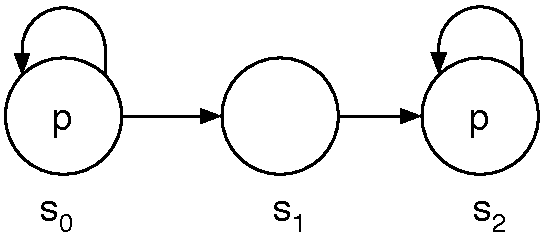
\includegraphics[width=.4\textwidth]
            {Figures/Kripke Structure Exercise 6.pdf}
    \caption{Kripe Structure, where $s₀⊧\mathbf{AFG} p$ holds, but
             $s₀⊧\mathbf{AFAG} p$ does not hold}
    \label{figure:Kripke_Structure_Exercise_6}
\end{figure}

\begin{figure}[htbp]
    \centering
        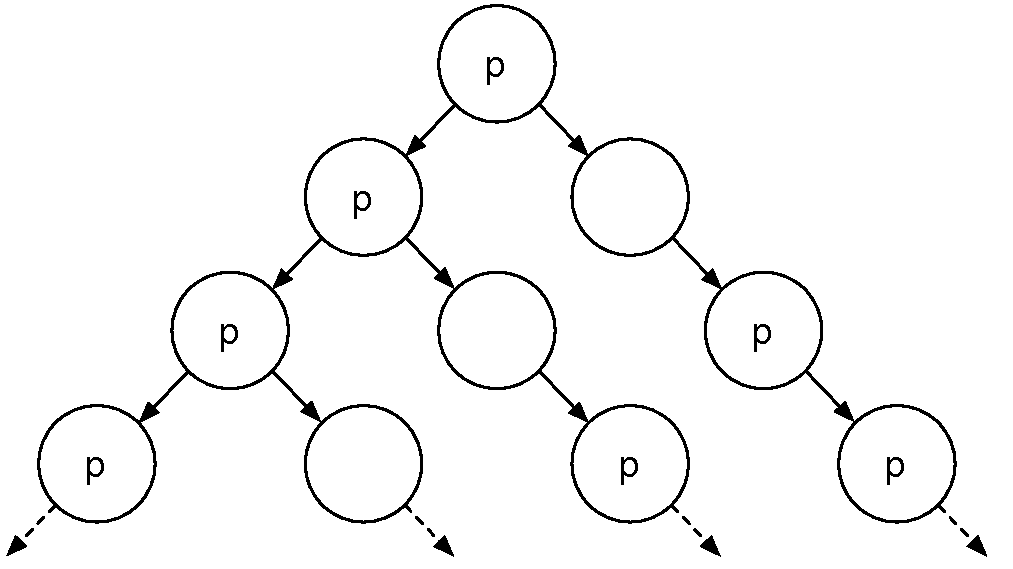
\includegraphics[width=.7\textwidth]
            {Figures/Computation Tree Exercise 6.pdf}
    \caption{Computation Tree for
             Figure~\ref{figure:Kripke_Structure_Exercise_6}}
    \label{figure:Computation_Tree_Exercise_6}
\end{figure}

\begin{description}[style=multiline, leftmargin=3cm]

    \item[$s₀⊧\mathbf{AF}(\mathbf{G} p)$] This formula specifies that in all
    paths sometimes in the future $p$ will hold globally. This is true for the
    given Kripke structure since we start in $s₀$ in which $p$ holds and either

        \begin{itemize}

            \item continue to stay in this state ($p$ holds globally) or

            \item go to $s₁$ immediately followed by state $s₂$ ($p$ holds
            globally).

        \end{itemize}

    \item[$s₀⊧\mathbf{AF}(\mathbf{AG} p)$] The formula specifies that
    sometimes in the future for all paths $\mathbf{AG} p$ (for all paths $p$
    must always be true) has to hold. This is not the case if we follow the
    path on the left in the computation tree for the Kripke Structure (see
    Figure~\ref{figure:Computation_Tree_Exercise_6}) since there is always a
    path on the right where $p$ does not hold for every state.

\end{description}

\subsection{Exercise 7}

Describe a simple model checker for CTL over Kripke structures in pseudocode.

\subsection{Exercise 8}

Find a translation of the $\mathbf{U}$ operator to propositional logic in
bounded model checking

\subsection{Exercise 9}

Show that all LTL properties have counterexamples which are either finite
paths or finite paths with a loop. Hint: Use the fact that LTL specifications
can be translated into Buechi automata.

\subsection{Exercise 10}

Give an LTL specification where the smallest counterexample is larger than the
number of states in the Kripke structure.

\subsection{Exercise 11}

Show how you can use SMV to solve chess problems. “Given a chess board, white
has a winning strategy in 3 moves.” How do you describe the board? What is
the specification?

% -- Bibliography -------------------------------------------------------------

% Set section format for bibliography
\titleformat{\section}{\sffamily\bfseries}{}{0pt}{}[{\color{aqua}\hrule}]
% Display bibliography
\printbibliography

\end{document}
